\documentclass[english, 11 pt, class=article, crop=false]{standalone}

\newcommand{\note}{Merk}
\newcommand{\notesm}[1]{{\footnotesize \textsl{\note:} #1}}
\newcommand{\ekstitle}{Eksempel }
\newcommand{\sprtitle}{Språkboksen}
\newcommand{\expl}{forklaring}

\newcommand{\vedlegg}[1]{\refstepcounter{vedl}\section*{Vedlegg \thevedl: #1}  \setcounter{vedleq}{0}}

\newcommand\sv{\vsk \textbf{Svar} \vspace{4 pt}\\}

%references
\newcommand{\reftab}[1]{\hrs{#1}{tabell}}
\newcommand{\rref}[1]{\hrs{#1}{regel}}
\newcommand{\dref}[1]{\hrs{#1}{definisjon}}
\newcommand{\refkap}[1]{\hrs{#1}{kapittel}}
\newcommand{\refsec}[1]{\hrs{#1}{seksjon}}
\newcommand{\refdsec}[1]{\hrs{#1}{delseksjon}}
\newcommand{\refved}[1]{\hrs{#1}{vedlegg}}
\newcommand{\eksref}[1]{\textsl{#1}}
\newcommand\fref[2][]{\hyperref[#2]{\textsl{figur \ref*{#2}#1}}}
\newcommand{\refop}[1]{{\color{blue}Oppgave \ref{#1}}}
\newcommand{\refops}[1]{{\color{blue}oppgave \ref{#1}}}
\newcommand{\refgrubs}[1]{{\color{blue}gruble \ref{#1}}}

\newcommand{\openmathser}{\openmath\,-\,serien}

% Exercises
\newcommand{\opgt}{\newpage \phantomsection \addcontentsline{toc}{section}{Oppgaver} \section*{Oppgaver for kapittel \thechapter}\vs \setcounter{section}{1}}


% Sequences and series
\newcommand{\sumarrek}{Summen av en aritmetisk rekke}
\newcommand{\sumgerek}{Summen av en geometrisk rekke}
\newcommand{\regnregsum}{Regneregler for summetegnet}

% Trigonometry
\newcommand{\sincoskomb}{Sinus og cosinus kombinert}
\newcommand{\cosfunk}{Cosinusfunksjonen}
\newcommand{\trid}{Trigonometriske identiteter}
\newcommand{\deravtri}{Den deriverte av de trigonometriske funksjonene}
% Solutions manual
\newcommand{\selos}{Se løsningsforslag.}
\newcommand{\se}[1]{Se eksempel på side \pageref{#1}}

%Vectors
\newcommand{\parvek}{Parallelle vektorer}
\newcommand{\vekpro}{Vektorproduktet}
\newcommand{\vekproarvol}{Vektorproduktet som areal og volum}


% 3D geometries
\newcommand{\linrom}{Linje i rommet}
\newcommand{\avstplnpkt}{Avstand mellom punkt og plan}


% Integral
\newcommand{\bestminten}{Bestemt integral I}
\newcommand{\anfundteo}{Analysens fundamentalteorem}
\newcommand{\intuf}{Integralet av utvalge funksjoner}
\newcommand{\bytvar}{Bytte av variabel}
\newcommand{\intvol}{Integral som volum}
\newcommand{\andordlindif}{Andre ordens lineære differensialligninger}


\usepackage[T1]{fontenc}
%\renewcommand*\familydefault{\sfdefault} % For dyslexia-friendly text
\usepackage{lmodern} % load a font with all the characters
\usepackage{geometry}
\geometry{verbose,paperwidth=16.1 cm, paperheight=24 cm, inner=2.3cm, outer=1.8 cm, bmargin=2cm, tmargin=1.8cm}
\setlength{\parindent}{0bp}
\usepackage{import}
\usepackage[subpreambles=false]{standalone}
\usepackage{amsmath}
\usepackage{amssymb}
\usepackage{esint}
\usepackage{babel}
\usepackage{tabu}
\makeatother
\makeatletter

\usepackage{titlesec}
\usepackage{ragged2e}
\RaggedRight
\raggedbottom
\frenchspacing

% Norwegian names of figures, chapters, parts and content
\addto\captionsenglish{\renewcommand{\figurename}{Figur}}
\makeatletter
\addto\captionsenglish{\renewcommand{\chaptername}{Kapittel}}
\addto\captionsenglish{\renewcommand{\partname}{Del}}


\usepackage{graphicx}
\usepackage{float}
\usepackage{subfig}
\usepackage{placeins}
\usepackage{cancel}
\usepackage{framed}
\usepackage{wrapfig}
\usepackage[subfigure]{tocloft}
\usepackage[font=footnotesize,labelfont=sl]{caption} % Figure caption
\usepackage{bm}
\usepackage[dvipsnames, table]{xcolor}
\definecolor{shadecolor}{rgb}{0.105469, 0.613281, 1}
\colorlet{shadecolor}{Emerald!15} 
\usepackage{icomma}
\makeatother
\usepackage[many]{tcolorbox}
\usepackage{multicol}
\usepackage{stackengine}

\usepackage{esvect} %For vectors with capital letters

% For tabular
\usepackage{array}
\usepackage{multirow}
\usepackage{longtable} %breakable table

% Ligningsreferanser
\usepackage{mathtools}
\mathtoolsset{showonlyrefs}

% index
\usepackage{imakeidx}
\makeindex[title=Indeks]

%Footnote:
\usepackage[bottom, hang, flushmargin]{footmisc}
\usepackage{perpage} 
\MakePerPage{footnote}
\addtolength{\footnotesep}{2mm}
\renewcommand{\thefootnote}{\arabic{footnote}}
\renewcommand\footnoterule{\rule{\linewidth}{0.4pt}}
\renewcommand{\thempfootnote}{\arabic{mpfootnote}}

%colors
\definecolor{c1}{cmyk}{0,0.5,1,0}
\definecolor{c2}{cmyk}{1,0.25,1,0}
\definecolor{n3}{cmyk}{1,0.,1,0}
\definecolor{neg}{cmyk}{1,0.,0.,0}

% Lister med bokstavar
\usepackage[inline]{enumitem}

\newcounter{rg}
\numberwithin{rg}{chapter}
\newcommand{\reg}[2][]{\begin{tcolorbox}[boxrule=0.3 mm,arc=0mm,colback=blue!3] {\refstepcounter{rg}\phantomsection \large \textbf{\therg \;#1} \vspace{5 pt}}\newline #2  \end{tcolorbox}\vspace{-5pt}}

\newcommand\alg[1]{\begin{align} #1 \end{align}}

\newcommand\eks[2][]{\begin{tcolorbox}[boxrule=0.3 mm,arc=0mm,enhanced jigsaw,breakable,colback=green!3] {\large \textbf{Eksempel #1} \vspace{5 pt}\\} #2 \end{tcolorbox}\vspace{-5pt} }

\newcommand{\st}[1]{\begin{tcolorbox}[boxrule=0.0 mm,arc=0mm,enhanced jigsaw,breakable,colback=yellow!12]{ #1} \end{tcolorbox}}

\newcommand{\spr}[1]{\begin{tcolorbox}[boxrule=0.3 mm,arc=0mm,enhanced jigsaw,breakable,colback=yellow!7] {\large \textbf{Språkboksen} \vspace{5 pt}\\} #1 \end{tcolorbox}\vspace{-5pt} }

\newcommand{\sym}[1]{\colorbox{blue!15}{#1}}

\newcommand{\info}[2]{\begin{tcolorbox}[boxrule=0.3 mm,arc=0mm,enhanced jigsaw,breakable,colback=cyan!6] {\large \textbf{#1} \vspace{5 pt}\\} #2 \end{tcolorbox}\vspace{-5pt} }

\newcommand\algv[1]{\vspace{-11 pt}\begin{align*} #1 \end{align*}}

\newcommand{\regv}{\vspace{5pt}}
\newcommand{\mer}{\textsl{Merk}: }
\newcommand{\mers}[1]{{\footnotesize \mer #1}}
\newcommand\vsk{\vspace{11pt}}
\newcommand\vs{\vspace{-11pt}}
\newcommand\vsb{\vspace{-16pt}}
\newcommand\sv{\vsk \textbf{Svar} \vspace{4 pt}\\}
\newcommand\br{\\[5 pt]}
\newcommand{\figp}[1]{../fig/#1}
\newcommand\algvv[1]{\vs\vs\begin{align*} #1 \end{align*}}
\newcommand{\y}[1]{$ {#1} $}
\newcommand{\os}{\\[5 pt]}
\newcommand{\prbxl}[2]{
\parbox[l][][l]{#1\linewidth}{#2
	}}
\newcommand{\prbxr}[2]{\parbox[r][][l]{#1\linewidth}{
		\setlength{\abovedisplayskip}{5pt}
		\setlength{\belowdisplayskip}{5pt}	
		\setlength{\abovedisplayshortskip}{0pt}
		\setlength{\belowdisplayshortskip}{0pt} 
		\begin{shaded}
			\footnotesize	#2 \end{shaded}}}

\renewcommand{\cfttoctitlefont}{\Large\bfseries}
\setlength{\cftaftertoctitleskip}{0 pt}
\setlength{\cftbeforetoctitleskip}{0 pt}

\newcommand{\bs}{\\[3pt]}
\newcommand{\vn}{\\[6pt]}
\newcommand{\fig}[1]{\begin{figure}
		\centering
		\includegraphics[]{\figp{#1}}
\end{figure}}

\newcommand{\figc}[2]{\begin{figure}
		\centering
		\includegraphics[]{\figp{#1}}
		\caption{#2}
\end{figure}}

\newcommand{\sectionbreak}{\clearpage} % New page on each section

\newcommand{\nn}[1]{
\begin{equation}
	#1
\end{equation}
}

% Equation comments
\newcommand{\cm}[1]{\llap{\color{blue} #1}}

\newcommand\fork[2]{\begin{tcolorbox}[boxrule=0.3 mm,arc=0mm,enhanced jigsaw,breakable,colback=yellow!7] {\large \textbf{#1 (forklaring)} \vspace{5 pt}\\} #2 \end{tcolorbox}\vspace{-5pt} }
 
%colors
\newcommand{\colr}[1]{{\color{red} #1}}
\newcommand{\colb}[1]{{\color{blue} #1}}
\newcommand{\colo}[1]{{\color{orange} #1}}
\newcommand{\colc}[1]{{\color{cyan} #1}}
\definecolor{projectgreen}{cmyk}{100,0,100,0}
\newcommand{\colg}[1]{{\color{projectgreen} #1}}

% Methods
\newcommand{\metode}[2]{
	\textsl{#1} \\[-8pt]
	\rule{#2}{0.75pt}
}

%Opg
\newcommand{\abc}[1]{
	\begin{enumerate}[label=\alph*),leftmargin=18pt]
		#1
	\end{enumerate}
}
\newcommand{\abcs}[2]{
	\begin{enumerate}[label=\alph*),start=#1,leftmargin=18pt]
		#2
	\end{enumerate}
}
\newcommand{\abcn}[1]{
	\begin{enumerate}[label=\arabic*),leftmargin=18pt]
		#1
	\end{enumerate}
}
\newcommand{\abch}[1]{
	\hspace{-2pt}	\begin{enumerate*}[label=\alph*), itemjoin=\hspace{1cm}]
		#1
	\end{enumerate*}
}
\newcommand{\abchs}[2]{
	\hspace{-2pt}	\begin{enumerate*}[label=\alph*), itemjoin=\hspace{1cm}, start=#1]
		#2
	\end{enumerate*}
}

% Oppgaver
\newcommand{\opgt}{\phantomsection \addcontentsline{toc}{section}{Oppgaver} \section*{Oppgaver for kapittel \thechapter}\vs \setcounter{section}{1}}
\newcounter{opg}
\numberwithin{opg}{section}
\newcommand{\op}[1]{\vspace{15pt} \refstepcounter{opg}\large \textbf{\color{blue}\theopg} \vspace{2 pt} \label{#1} \\}
\newcommand{\ekspop}[1]{\vsk\textbf{Gruble \thechapter.#1}\vspace{2 pt} \\}
\newcommand{\nes}{\stepcounter{section}
	\setcounter{opg}{0}}
\newcommand{\opr}[1]{\vspace{3pt}\textbf{\ref{#1}}}
\newcommand{\oeks}[1]{\begin{tcolorbox}[boxrule=0.3 mm,arc=0mm,colback=white]
		\textit{Eksempel: } #1	  
\end{tcolorbox}}
\newcommand\opgeks[2][]{\begin{tcolorbox}[boxrule=0.1 mm,arc=0mm,enhanced jigsaw,breakable,colback=white] {\footnotesize \textbf{Eksempel #1} \\} \footnotesize #2 \end{tcolorbox}\vspace{-5pt} }
\newcommand{\rknut}{
Rekn ut.
}

%License
\newcommand{\lic}{\textit{Matematikken sine byggesteinar by Sindre Sogge Heggen is licensed under CC BY-NC-SA 4.0. To view a copy of this license, visit\\ 
		\net{http://creativecommons.org/licenses/by-nc-sa/4.0/}{http://creativecommons.org/licenses/by-nc-sa/4.0/}}}

%referances
\newcommand{\net}[2]{{\color{blue}\href{#1}{#2}}}
\newcommand{\hrs}[2]{\hyperref[#1]{\color{blue}\textsl{#2 \ref*{#1}}}}
\newcommand{\rref}[1]{\hrs{#1}{regel}}
\newcommand{\refkap}[1]{\hrs{#1}{kapittel}}
\newcommand{\refsec}[1]{\hrs{#1}{seksjon}}

\newcommand{\mb}{\net{https://sindrsh.github.io/FirstPrinciplesOfMath/}{MB}}


%line to seperate examples
\newcommand{\linje}{\rule{\linewidth}{1pt} }

\usepackage{datetime2}
%%\usepackage{sansmathfonts} for dyslexia-friendly math
\usepackage[]{hyperref}



\begin{document}
\newpage
\section{Indeksregning}
\subsection{Introduksjon}
\parbox{0.6\linewidth}{Innen økonomi er \textit{indekser} forholdstall som forteller hvor mye størrelser har forandret seg. For eksempel kostet kroneisen ca 0,75\,kr (!) da den ble lansert i 1953, mens den i 2021 kostet ca 27\,kr. Forholdet mellom prisen i 2021 og i 1953 er da
	\[ \frac{\text{pris 2021}}{\text{pris 1953}}=\frac{27}{0,75}= 36 \]
}
\parbox[r]{0.3\linewidth}{
\includegraphics[scale=2]{kr}}\\[2pt]
I denne sammenhengen  er tallet 36 en indeks for prisendringen på kroneis mellom 1953 og 2021.

\begin{comment}
	\regv 
	\reg[Indeks]{\vsb
	\[ \frac{\text{verdi 1}}{\text{verdi 2}}\cdot 100 = \text{indeks} \]
	}
	\eks[1]{
	En vare kostet 15\,kr i 2017 og 5\,kr i 1990. Regn ut indeksen for prisendringen fra 2017 til 1990.
	
	\sv 
	Vi deler prisen fra 2017 med prisen fra 1990 og ganger medd 100:
	\[ \frac{15}{5}\cdot 100 = 300 \]
	Indeksen er altså 300.
	}
	\eks[2]{
	En vare kostet i 2000 10 kr. In
	}
\end{comment}
\subsection{Konsumprisindeks og basisår}
\textit{Konsumprisindeksen} (KPI) er en indeks som beskriver et sammenlignbart prisnivå på varer og tjenester som en typisk husstand i Norge bruker penger på i løpet av et år. Disse varene er \vs

\parbox[t]{0.49\linewidth}{\begin{itemize}
		\item Matvarer og alkoholfrie drikkevarer
		\item Alkoholholdige drikkevarer og tobakk
		\item Klær og skotøy
		\item Bolig, lys og brensel
		\item Møbler, husholdningsartikler og vedlikehold av innbo
		\item Helsepleie
\end{itemize}}
\parbox[t]{0.49\linewidth}{\begin{itemize}
		\item Transport
		\item Post- og teletjenester
		\item Kultur og fritid
		\item Utdanning
		\item Hotell- og restauranttjenester
		\item Elektrisitet
\end{itemize}}
For å sammenligne noe må man alltid ha et utgangspunkt, og konsumprisindeksen tar utgangspunkt i prisnivået på de nevnte varene/tjenestene i året 2015. 2015 kalles da \textit{basisåret}\footnote{Hvilket år som er basisår forandrer seg med tiden. Før 2015 ble basisår var 1998 det.}, og i dette året er indeksen satt til 100.\regv
\reg[Basisår]{I et basisår er verdien til indeksen 100. For konsumprisindeksen er 2015 basisåret.}\vsk

Tabellen under viser samlet KPI for de 10 siste årene:
\begin{center}
	\begin{tabular}{c|c}
		År &  KPI \\ \hline
		2020 & 112,2\\
		2019 & 	110,8\\
		2018 &  112,2 \\
		2017&	105,5\\
		2016&	103,6\\
		2015&	100\\
		2014&	97,9\\
		2013&	95,9\\
		2012&	93,9\\
		2011&	93,3\\
	\end{tabular}
	\captionof{table}{Kunsumprisindeksen for årene 2010-2021. Tall hentet fra \net{https://www.ssb.no/priser-og-prisindekser/konsumpriser/statistikk/konsumprisindeksen}{SSB}. \label{KPI}}
\end{center}
Ut ifra tabellen kan vi for eksempel lese dette:
\begin{itemize}
	\item Da KPI for 2017 er 105,5\,, har prisene steget med 5,5\% siden 2015.
	\item Da KPI i 2011 er 93,3\,, var prisene 7,7\% lavere i 2011 enn i 2015.
\end{itemize}
\reg[Prosentvis endring fra basisår]{\vs
\[ \text{indeks}-100=\text{prosentvis endring fra basisår} \]
}
\eks[1]{
I juli 2021 var KPI for	matvarer 109,4. Hvor mye har prisen på matvarer endret seg sammenlignet med basisåret?

\sv $ {109,4-100=9,4}  $. Prisen på matvarer har altså økt med 9,4\% sammenlignet med basisåret.
}
\newpage
\eks[2]{
I juli 2021 var KPI for sko 98,0. Hvor mye har prisen på sko endret seg sammenlignet med basisåret?

\sv 
$ 98,0-100=-2 $. Prisen på sko har altså blitt redusert med 2\% sammenlignet med basisåret.  
}
\subsection{Kroneverdi}
Vi har nevnt at en kroneis kostet 0,75 \,kr i 1953 og 27\,kr i 2021. Når vi ved to tidspunkt må betale \textsl{forskjellig} pris på den \textsl{samme} varen skyldes det ofte at \textit{kroneverdien} har forandret seg;\textsl{ 1\enh{kr} i 1957 var mer verd  enn 1\enh{kr} i 2021.
}\vsk

Kroneverdien for et gitt år regnes ut ifra KPI til basisåret (100): \regv
	
\reg[Kroneverdi \label{kroneverdi}]{\vs
\[ \text{kroneverdi}=\frac{100}{\text{KPI}} \]
{\footnotesize\mer Kroneverdien for basisåret (2015) er 1.}
}
\eks[1]{
KPI i 2012 var 93,9. Regn ut kroneverdien i 2012.

\sv \vs
\algv{
\text{kroneverdi i 2012} &= \frac{100}{93,9}\\
&\approx 1,06
}
Dette betyr at 1\,kr i 2012 tilsvarer 1,06\enh{kr} i basisåret.
} \vsk

\info{Obs!}{
Ordet \textit{kroneverdi} brukes også når man sammenlikner verdien av 1\enh{kr} opp mot verdien av utenlandsk valuta. Kroneverdi ut ifra et basisår og kroneverdi ut ifra en valuta er ikke det samme.
}

\reg[Realverdi \label{realverdi}]{
Realverdien til en pengesum er hvor mye en pengesum ville vært verd i basisåret.	
\[ \text{realverdi} = \text{opprinnelig verdi}\cdot \text{kroneverdi} \]
}
\eks{
I 1928 var KPI 3,2 og i 2020 var KPI 112,2. Hva hadde størst realverdi, 10\,000\enh{kr} i 1928 eller 350\,000\enh{kr} i 2020? 

\sv
Vi har at
\algv{
\text{kroneverdi i 1928} &= \frac{100}{3,2}
}
Altså er
\alg{
\text{verdien av 10\,000\enh{kr} fra 1928 i basisår}&= 10\,000\enh{kr}\cdot \frac{100}{3,2} \\
&= 312\,500 \enh{kr}
}
Videre er
\algv{
	\text{kroneverdi i 2012} &= \frac{100}{112,2}
}
Altså er
\alg{
	\text{verdien av 350\,000\enh{kr} fra 1928 i basisår}&= 350\,000\cdot \frac{100}{112,2} \\
	&\approx 311\,943\enh{kr}
}
Altså var 10\,000\enh{kr} mer verd i 1928 enn det 350\,000\enh{kr} var verd i 2020.
}
\subsection{Reallønn og nominell lønn}
Hvor god \textit{råd} vi har avhenger av hvor mye vi tjener og hva prisnivået er. Tenk at du  hadde en årslønn på 500\,000\,kr i både 2020 og i 2019. \hyperref[KPI]{\textsl{Tabell \ref*{KPI}}} forteller oss da at du hadde du best råd i 2019, fordi da var prisnivået (KPI) lavere enn i 2020. \vsk

At prisnivået har blitt høgere er det samme som at kroneverdien har blitt lavere. Dette betyr igjen at hvis lønnen din var den samme i 2019 og 2020, er \textsl{realverdien} til lønnen din høgere i 2019 enn i 2020. Den opprinnelige lønnen og realverdien til lønnen er så mye brukt i statistikk at de har fått egne navn:\regv

\reg[Reallønn og nominell lønn\label{realnomonn}]{
Nominell lønn er lønn  mottat et gitt år. \vsk

Reallønnen er realverdien til den nominelle lønnen. 	
}
\eks{
I 2016 tjente Per 450\,000 kr, mens i 2012 tjente han 420\,000 kr. I 2016 var $ {\text{KPI}=103,6} $, mens i 2012 var $ {\text{KPI}=93,9} $. I hvilket av disse årene hadde Per best råd?

\sv
For å finne ut hvilket av årene Per hadde best råd i, sjekker vi hvilket år han hadde høgest reallønn\footnote{KPI-verdiene i utregningen henter vi fra \hyperref[KPI]{\textsl{Tabell 1}}.} (se \rref{realverdi}):
\alg{
\text{reallønn i 2016}&= 450\,000\cdot\frac{100}{103,6}\enh{kr} \\
& \approx 434\,363 \enh{kr}\vn
\text{reallønn i 2012}&= 420\,000\cdot\frac{100}{93,9} \\
& \approx 447\,284 \enh{kr}
}
Reallønnen til Per var altså høgest i 2012, derfor hadde han bedre råd da enn i 2016.
}
\newpage
\reg[Verdi som følger indeks]{
En verdi er sagt å ha \textit{fulgt indeks} hvis verdi og indeks ved to tidspunkt er like.
\[ \frac{\text{verdi ved tidspunkt 1}}{\text{indeks ved tidspunkt 1}} = \frac{\text{verdi ved tidspunkt 2}}{\text{indeks ved tidspunkt 2}} \]
}

\eks[1]{
	Tabellen under viser en oversikt over prisen registrert i en butikk på to varer ved to forskjellige tidspunkt. 
	\begin{center}
		\begin{tabular}{r|r|r|}
			& \textbf{2010} & \textbf{2020}	\\ \hline
			sjokolade & 11,00\enh{kr} & 13,40\enh{kr} \\
			brus	& 12,50\enh{kr} & 19,00\enh{kr}
		\end{tabular}
	\end{center}
I 2010 var KPI 92,1 og i 2020 var KPI 12,2.
Har prisen på noen av varene fulgt indeks?

\sv

Vi har at
\alg{
\frac{\text{pris på sjokolade i 2010}}{\text{KPI i 2010}} &= \frac{11}{92,1}\approx 0,119 \vn
\frac{\text{pris på sjokolade i 2020}}{\text{KPI i 2020}} &= \frac{13,40}{112,1}\approx 0,119
}
Videre er
\alg{
	\frac{\text{pris på brus i 2010}}{\text{KPI i 2010}} &= \frac{12,5}{92,1}\approx 0,136 \vn
	\frac{\text{pris på brus i 2020}}{\text{KPI i 2020}} &= \frac{19}{112,1}\approx 0,169
}
Altså er det rimelig å si at prisen for sjokolade har fulgt indeks, mens prisen for brus ikke har gjort det.
}

\section{Lån og sparing}
\subsection{Lån}
Noen ganger har vi  ikke nok penger til å kjøpe det vi ønsker oss, og må derfor ta opp et lån fra en bank. Banken gir oss da en viss \textit{lånesum} mot at vi betaler tilbake denne, og \textit{renter}, i løpet av en bestemt tid. Det vanligste er at vi underveis betaler banken det som kalles \textit{terminbeløp}, som på sin side består av \textit{avdrag} og renter. Det vi til enhver tid skylder banken kaller vi \textit{gjelden}. \vsk

Si at en bank låner  oss 100\,000\,kr, som da er lånesummen. Lånet skal tilbakebetales i løpet av 5 år, med ett terminbeløp hvert år, og renten er 10\%. Det finnes forskjellige måter å betale tilbake et lån på, men følgende vil som regel gjelde:
\begin{itemize}
	\item \textbf{Summen av alle avdragene skal tilsvare lånesummen}.\os
	 For å gjøre det enkelt i vårt eksempel, bestemmer vi oss for å betale tilbake lånet med like avdrag hvert år. Siden 100\,000 kr skal fordeles likt over 5 år, må det årlige avdraget bli $ \frac{100\,000}{5}\enh{kr}=20\,000 $\,kr.
	\item \textbf{Det man betaler i avdrag skal trekkes fra gjelden.}\os
	
	Startgjelden er 100\,000\enh{kr}, men det første året betaler vi 20\,000\,kr i avdrag, og da blir gjelden $100\,000\enh{kr}-20\,000\enh{kr} =80\,000\enh{kr} $. Det andre året betaler vi nye 20\,000\,kr, og da blir gjelden $ 80\,000\enh{kr}-20\,000\enh{kr} =60\,000\enh{kr}  $. Og slik fortsetter det de neste tre årene.
	\item \textbf{Renter skal beregnes av gjelden.}\os 
	Siden gjelden det første året er 100\,000\,kr, må vi betale \\${ 100\,000\enh{kr}\cdot0,1=10\,000\enh{kr} } $ i renter. Siden gjelden det andre året er 80\,000\,kr må vi betale ${ 80\,000\enh{kr}\cdot0,1=8\,000\enh{kr} } $ i renter.  Og slik fortsetter det de neste tre årene.
	
	\item \textbf{Terminbeløpet er summen av avdraget og rentene}.\os
	
	Av første og tredje punkt får vi at\os
	\centering
	\begin{tabular}{c| c |c}
		 & 1. år & 2. år \\ \hline
		Terminbeløp 
			& $\begin{matrix}
			20\,000\enh{kr} +10\,000\enh{kr}\\
			= \\
			30\,000\enh{kr}
			\end{matrix} $  
				& $\begin{matrix}
					20\,000\enh{kr} +80\,000\enh{kr}\\
					= \\
					28\,000\enh{kr}
					\end{matrix} $ 
	\end{tabular}\os
\raggedright 
Og slik fortsetter det de neste tre årene.
\item \textbf{Lånet er fullført når gjelden er lik 0\enh{kr} og alle renter er betalt.}\os
Hvis vi har betalt avdrag lik 20\,000\enh{kr} i 5 år, er gjelden 0\enh{kr}. Har vi da betalt alle rentene også, er lånet fullført. \os

{\footnotesize\mer Du har alltid rett til å betale større avdrag enn det som først er avtalt. Betaler du hele gjelden vil lånet avsluttes så lenge eventuelle renter også er betalt.}
\end{itemize}\vsk
\textbf{Serielån og annuitetslån}\os
To vanlige typer lån er \textit{serielån} og \textit{annuitetslån}. Lånet fra eksempelet vi akkurat har sett på er et serielån fordi avdragene er like store. Hvis terminbeløpene hadde vært like store, ville det isteden vært et annuitetslån. Hvis lånesum, rente og nedbetalingstid er lik, vil et serielån alltid medføre minst utgifter totalt sett. For privatpersoner er det likevel veldig populært å velge annuitetslån på grunn av at det er lettere å planlegge økonomien når man betaler det samme beløpet hver gang. \vsk

\textbf{Kredittkort}\os
\prbxl{0.6}{Kredittkort er et betalingskort som er slik at hvis du f.eks. bruker kortet for å betale 10\,000\,kr, så låner du pengene fra banken. Etter en tid som er avtalt med banken vil den kreve renter av gjelden din. Til hvilken tid du betaler denne gjelden }\qquad
\parbox{0.3\linewidth}{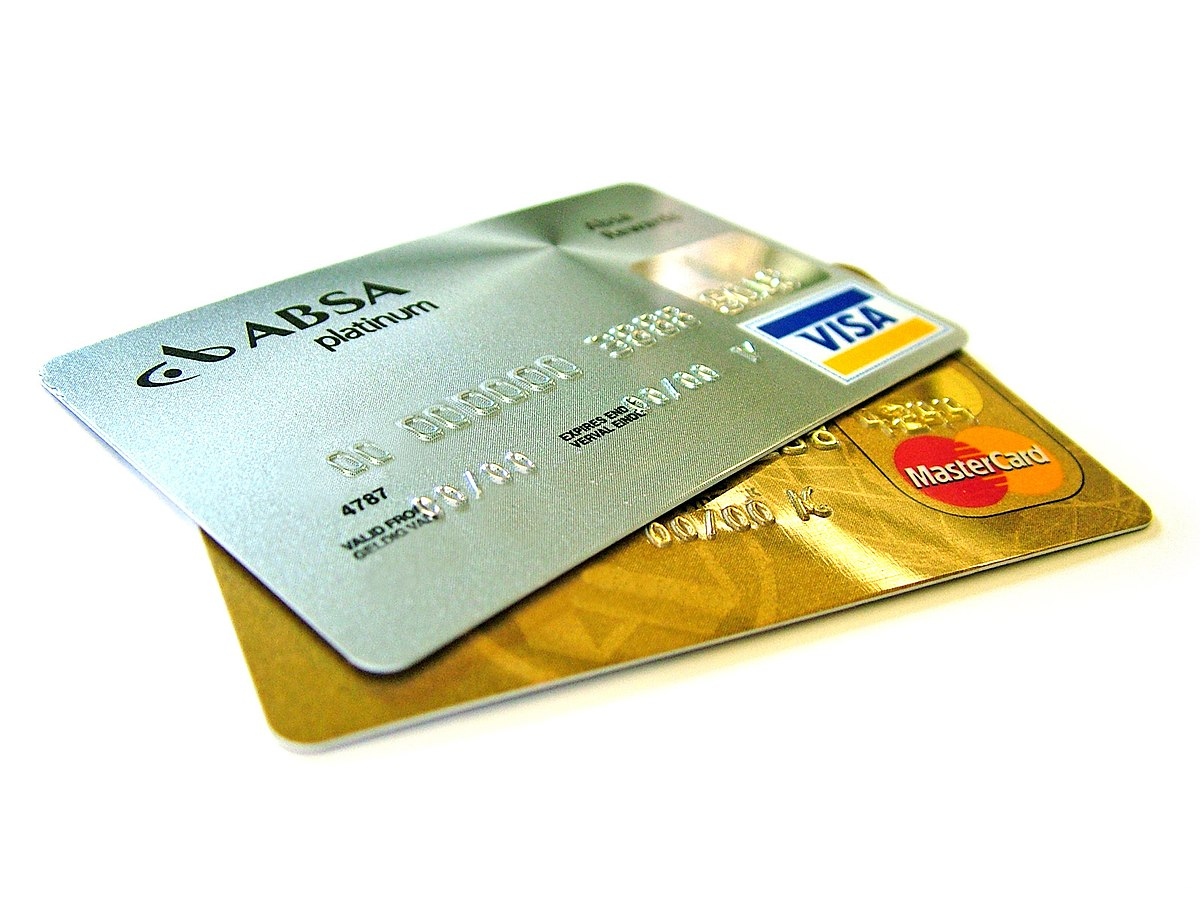
\includegraphics[scale=0.1]{kred}}\\[-3pt]
er delvis opp til deg selv, men generelt har kredittkort veldig høge renter, så det lureste er å betale før rentekravet har startet!
\regv
\reg[Lån]{
\renewcommand{\arraystretch}{1.5}
\begin{tabular}{>{\bfseries}r l}
	lånesum & Beløpet vi låner av banken. \\
	gjeld & Det vi til enhver tid skylder banken. \\
	rente & Prosentandel av gjeld som skal betales.\\
	avdrag & Det vi betaler ned på gjelden.  \\
	& Summen av avdragene tilsvarer lånesummen.\\
	&ny gjeld $ =  $ gammel gjeld $ - $ avdrag \\
	renter & gjeld $ \cdot $ rente \\
	terminbeløp & avdrag $ + $ renter \\
	serielån & Lån hvor avdragene er like store. \\
	annuitetslån & Lån hvor terminbeløpene er like store. \\
	kredittkort & Betalingskort som oppretter et lån fra banken.
\end{tabular}
}
\newpage
\eks[1]{
Fra en bank låner du 300\,000 kr med 3\% årlig rente. Lånet skal betales tilbake som et serielån med 5 årlige terminbeløp. \os
\textbf{a)} Hva blir det årlige avdraget?\os
\textbf{b)} Hva er gjelden din etter at du har betalt tredje terminbeløp?\os
\textbf{c)} Hvor mye må du betale i renter ved fjerde terminbeløp?\os
\textbf{d)} Hvor stort blir det fjerde terminbeløpet?\os 


\sv
\textbf{a)} Siden 300\,000\,kr skal betales over 5 år, blir det årlige avdraget
\[ \frac{300\,000\enh{kr}}{5}=60\,000\enh{kr} \]
\textbf{b)} Når tredje terminbeløp er betalt, har du betalt tre avdrag. Det betyr at gjelden din er
\alg{
300\,000-60\,000\cdot3 &= 300\,000-180\,000 \\
&= 120\,000
}
Altså 120\,000\,kr.\os

\textbf{c)} Ut ifra oppgave b) vet vi at gjelden er 180\,000 kr når fjerde terminbeløp skal betales. 3\% av gjelden blir da
\[ 180\,000\cdot0,03=5\,400 \]
Altså 5\,400 kr.\os
\textbf{d)} Terminbeløpet tilsvarer avdrag pluss renter. Ut ifra oppgave a) og c) vet vi da at det fjerde terminbeløpet blir
\[ 60\,000\enh{kr}+5\,400\enh{kr} =65\,400\enh{kr}\]}
\newpage
\eks[2]{
Fra en bank låner du 100\,000\,kr med 6,4\% årlig rente. Lånet skal betales tilbake som et annuitetslån over 5 år, og banken har da regnet ut at terminbeløpet blir 24\,000\enh{kr}.\os

Regn ut avdrag og renter for det første terminbeløpet.

\sv
Det første året er gjelden 100\,000\,kr, i renter må du betale 6,4\% av denne:
\[ 100\,000\cdot0,064=6\,400 \]
Altså må du betale 6\,400\,kr i renter det første året.\vsk

Vi har at
\[ \text{terminbeløp}=\text{avdrag}+\text{renter} \]
Dermed er
\[ {\text{avdrag}=\text{terminbeløp}-\text{avdrag}} \]
\[ =24\,000-6400=17\,600 \]
Altså må du betale 17\,600\enh{kr} i avdrag det første året.
}
\newpage
\subsection{Sparing; innskuddsrente og forventet avkastning}
\subsubsection{Innskuddsrente}
Vi har sett at vi må betale renter når vi låner penger av en bank, men hvis vi i steden setter penger (gjør et innskudd) i en bank  \textsl{får} vi renter: \regv
\reg[Innskuddsrente]{
Innskuddsrente er en prosentvis økning av pengene du har i banken, gjentatt over faste tidsintervaller (månedlig, årlig o.l.) 
}
\eks[1]{
Du setter inn 20\,000\,kr i en bank som gir 2\% årlig sparerente. Hvor mye penger har du i banken etter 8 år? 

\sv
For å beregne innskuddsrenter kan vi anvende \rref{progjen}. Siden renten er 2\%, er vekstfaktoren 1,02. Originalverdien er 20\,000 og antall endringer (tiden) er 8:
\[ 20\,000\cdot1,02^8\approx 23\,433 \]
Du har altså ca. 23\,433\,kr i banken etter 8 år med sparing.
}
\subsubsection{Forventet avkastning}
En annen måte å spare penger på, er å investere i et aksjefond. Da vil man snakke om \textit{forventet avkastning}:\regv
\reg[Forventet avkastning]{
Forventet avkastning angir en \textsl{forventet} prosentvis økning av en investering, gjentatt over faste tidsintervaller.
}
\newpage
\eks[1]{
Du investerer 15\,000 i et aksjefond som forventer 5\% årlig avkastning. Hvor mye penger er investeringen verd etter 8 år ved en slik avkastning?

\sv
Også for forventet avkastning kan vi bruke \rref{progjen}. Vekstfaktoren er 1,05, originalverdien er 15\,000 og antall endringer (tiden) er 8:
\[ 15\,000\cdot1,05^8\approx22\,162 \]
Etter 8 år er det forventet at investeringen er verdt 22\,162\enh{kr}.
}
\vsk

\info{Spare med innskuddsrente eller aksjefond?}{
Som regel er forventet avkastning på et aksjefond høgere enn innskudsrenten du får i en bank, men ulempen er at forventet avkastning ikke gir noen garantier. Forventet avkastning oppgir bare økningen eksperter antar vil skje. Er du heldig blir økningen høgere, er du uheldig blir den lavere, og kan til og med føre til en \textsl{reduksjon} av investeringen din. I verste fall, rett nok i ekstremt sjeldne tilfeller, kan hele investeringen din ende opp med å bli verd 0\enh{kr}. \vsk

Innskuddsrenten kan også forandre seg noe med tiden, men den kan aldri føre til en reduksjon av investeringen din.
}
\begin{comment}
	\eks[2]{Du betaler 27\,000\,kr med et kreddittkort som krever 1,4\% rente for hver måned du betaler for seint.\os
	
	\textbf{a)} Hvor mye har du i gjeld to år etter for sein betaling?\os
	\textbf{b)} Hva er den årlige renten ved for sein betaling?
	
	\sv
	\textbf{a)} Siden renten er 1,4\%, er vekstfaktoren 1,014. Siden renten er månedlig må vi måle tiden i måneder, og to år er $ {2\cdot12=24} $ måneder. Siden starverdien er 27\,000, får vi:
	\[ 27\,000\cdot1,014^8\approx 37\,649 \]
	Etter to år har du altså ca 37\,649\,kr i gjeld.\os
	
	\textbf{b)} Siden ett år er det samme som 12 måneder blir vekstfaktoren gitt ved: 
	\[ 1,014^{12} \approx1.182\]
	}
\end{comment}


\section{Skatt}
Om du har en inntekt, må du som regel betale en del av disse pengene til staten. Disse pengene kalles \textit{skatt} (og noen ganger \textit{avgift}). Hensikten med skatt er at staten skal ha råd til å gi innbyggerne tilbud som skole, helsetjenester og mye mer. I dag blir blir skatten i stor grad beregnet av datasystemer, men det er ditt ansvar å sjekke at beregningene er riktige $ - $ og da er det viktig å forstå hvordan skattesystemet fungerer.\vsk

\info{Obs!}{I eksamensoppgaver og i virkeligheten vil du fort oppdage at skattesystemer er presentert på en litt annen måte enn i denne boka. Dette er blant annet fordi skattereglene kan forandre seg fra år til år, og i denne boka har vi tatt utgangspunkt i skattereglene for 2018. Det viktigste er ikke at du husker spesifikt disse reglene, men at du lærer deg hva som menes med begrepene \textit{bruttolønn, fradrag, skattegrunnlag, trygdeavgift} og \textit{nettolønn}.}
\subsection{Bruttolønn, fradrag og skattegrunnlag}
\prbxl{0.68}{De fleste må betale 23\% av det som kalles \textit{skattegrunnlaget}, som er \textit{bruttolønnen} minus \textit{fradrag}. Bruttolønnen er lønnen du mottar fra arbeidsgiver, mens fradrag kan være mye forskjellig. \textit{Personfradrag} og  \textit{minstefradrag} er noe alle skattebetalere får, i tillegg kan man }\qquad
\prbxr{0.22}{Skattegrunnlag kalles noen ganger \textit{trekkgrunnlag}.} \\[-16pt]

\prbxl{0.66}{blant annet få fradrag hvis man betaler \textit{fagforeningskontigent} eller har gitt penger til veldedige formål.}\qquad
\prbxr{0.24}{Fagforeningskontigent er det du betaler for å være med i en \net{https://no.wikipedia.org/wiki/Fagforening}{fagforening}.}\regv

\reg[Bruttolønn, fradrag og skattegrunnlag]{\vs
\begin{center}
	\begin{tabular}{c r}
		\phantom{xxxxx} &bruttolønn	\\
		$ - $ & fradrag \\ \hline
		$ = $ & skattegrunnlag \\ \hline
	\end{tabular}
\end{center}
}
\newpage
\eks{
Bruttolønnen til Magnus er 500\,000\,kr. Han får 56\,000\,kr i personfradrag 97\,600\,kr i minstefradrag, i tilleg betaler han 1\,000\,kr for årlig medlemskap i fagforeningen \textsl{Tekna}.\os
Hva må Magnus betale hvis han skatter 23\% av skattegrunnlaget?

\sv
Vi starter med å regne ut skattegrunnlaget, som er bruttolønnen minus fradragene:
\begin{center}
	\begin{tabular}{c r l}
	\phantom{xxxxx}	& 500\,000 & bruttolønn	\\
		$ - $& 56\,000 & personfradrag \\
		$ - $& 97\,600 & minstefradrag \\
		$ - $& 1\,000 &fagforeningskontigent \\ \hline
		$ = $ &345\,400 & skattegrunnlag \\ \hline
	\end{tabular}
\end{center}
}

\subsection{Trygdeavgift}
Alle lønnsmottakere må også betale \textit{trygdeavgift}. Dette er en inntekt staten bruker til å dekke \net{https://no.wikipedia.org/wiki/Folketrygden_(Norge)}{Folketrygden}. Hva man må betale i trygdeavgift kommer an på hvor gammel du er og hvilken type inntekt du har, men her skal vi bare bry oss om det man må betale for lønn fra en arbeidsgiver. Da er trygdeavgiften avhengig av alderen: \regv
\reg[Trygdeavgift]{\vs
\begin{center}
	\begin{tabular}{l| r}
		alder & trygdeavgift\\ \hline
		17-69 år &	8,2 \% \\
		under 17 år eller over 69 år &	5,1\%
	\end{tabular}
\end{center}
Trygdeavgiften skal beregnes av bruttolønnen.
}
\newpage
\eks{
Jonas og bestemoren hans, Line, har begge 150\,000\,kr i lønn. Jonas er 18 år og Line er 71 år.\os
\textbf{a)} Hva må Jonas betale i trygdeavgift?\os
\textbf{b)} Hva må Line betale i trygdeavgift?

\sv
\textbf{a)} Siden Jonas er mellom 17 år og 69 år, skal han betale 8,2\% trygdeavgift:
\[ 150\,000\cdot0,082=12\,300 \]
Altså skal Jonas betale 12\,300\,kr i trygdeavgift.
Sidan Line er over 69 år, skal hun betale 5,1\% trygdeavgift:
\[ 150\,000\cdot0,051=7\,650\]
Altså skal Line betale 7\,650\,kr i trygdeavgift.
}
\subsection{Trinnskatt \label{trinnskatt}}
Av lønnen din må du også betale en viss prosent av forskjellige intervall, dette kalles \textit{trinnskatt}:\regv
\reg[Trinnskatt]{\vs
\begin{center}
	\begin{tabular}{l| r |r}
		& Intervall & Skatt \\ \hline
		Trinn 1	& 169 000\,-\,237 900\,kr&	1,4\% \\
		Trinn 2	& 237 900\,-\,598 050\,kr&	3,3\%  \\
		Trinn 3	& 598 050\,-\,962 050\,kr&	12,4\%  \\
		Trinn 4	& Over 962 050\,kr	&15,4\% 
	\end{tabular}
\end{center}
Trinnskatt beregnes av bruttolønnen.
}
\newpage
\eks{
Hvis du tjener 550\,000 blir utregningen av trinnskatt slik:

\begin{center}
\small
		\begin{tabular}{c|l}
\multirow{3}{*}{Trinn 1} 
\\[-14pt] \hline \\
& Da hele lønnen er over 237\,900\,kr, må du betale \\
&skatt av  ${(237\,900-169\,000)\enh{kr} = 68\,900\enh{kr}}  $. \os
& Skatt for trinn 1 blir da $ 68\,900\enh{kr}\cdot0,014\approx 965\enh{kr} $.\os \hline \\
\multirow{4}{*}{Trinn 2} 
& Da 550\,000\,kr er over 237\,900\,kr, men under 598\,050\,kr,\\
& må du betale skatt av ${(550\,000-237\,900)\enh{kr} = 312\,100\enh{kr}}  $.  \os
& Skatt for trinn 2 blir da $ 312\,100\enh{kr}\cdot0,033\approx 10\,299\enh{kr} $. \os \hline \\
\multirow{2}{*}{Totalt} 
& Totalt må du betale $ {965\enh{kr}+10\,299\enh{kr}=11\,264\enh{kr}} $\\
& i trinnskatt.
	\end{tabular}
\end{center}
}
\newpage
\subsection{Nettolønn}
Det du sitter igjen med etter å ha betalt skatt, trygdeavgift og fagforeningskontigent kalles \textit{nettolønnen}. Med tanke på de tre tidligere delseksjonene kan vi sett opp et regnestykke som dette: \regv
\reg[Nettolønn]{
\begin{center}\vsb
	\begin{tabular}{c r}
	\phantom{xxxxxxx}	& Bruttolønn \\
		$ - $ & Fagforeningskontigent\\ 
		$ - $& 23\% skatt \\
		$ - $ & Trygdeavgift \\
		$ - $ & Trinnskatt \\ \hline
		$ = $ & Nettolønn \\ \hline
	\end{tabular}
\end{center}
}
\eks{
Emblas bruttolønn er 550\,000\,kr. Hun betaler 1500\,kr i året for medlemskap i \textsl{LO} (Norges største fagforening) og har 409\,900\enh{kr} som skattegrunnlag. Embla er 28 år.\os

Hva er nettolønnen til Embla?

\sv \vsb
\begin{center}
	\begin{tabular}{c r l}
		\phantom{xxxxxxx} & 550\,000	& Bruttolønn \\
		$ - $ & 1\,500\, & Fradrag for fagforening \\
		$ - $& $ 93\,127 $& 23\% av skattegrunnlaget \\
		$ - $ & 45\,100 & 8,2\% av bruttolønn \\
		$ - $ & 11\,264 & Total skatt for trinn 1 og 2 \\ \hline
		$ = $ & 399\,009& Nettolønn \\ \hline
		
	\end{tabular}
\end{center}
(Den totale trinnskatten har vi hentet fra utregningen i \textsl{Eksempel 1} fra \hyperref[trinnskatt]{\textsl{delseksjon \ref*{trinnskatt}}}.)\vsk

Embla har altså 399\,009\,kr i nettolønn.
}
\section{Budsjett og regnskap}
\subsection{Budsjett \label{budsjett}}
Når man skal planlegge økonomien sin, kan det være lurt å sette opp en oversikt over det man forventer av inntekter og utgifter. En slik oversikt kalles et \textit{budsjett}. Når man regner ut hva inntekter minus utgifter er, finner man et \textit{resultat}. Er tallet positivt går man med \textit{overskudd}, er tallet negativt går man med \textit{underskudd}.

\regv
\eks{
Lisa vil lage en oversikt over sine månedlige inntekter og utgifter, og kommer fram til dette:
\begin{itemize}
	\item Hun tar på seg kveldsvakter på en gamlehjem. Av dette forventer hun ca. 4\,000\enh{arg1} i nettolønn. \\
	\item Hun bruker ca. 4\,500 kr i måneden på mat.
	\item Hun får 4\,360\enh{kr} i borteboerstipend.
	\item Hun bruker ca. 1\,200\enh{kr} på klær, fritidsaktiviteter o.l.
\end{itemize}
Sett opp et månedsbudsjett for Lisa.

\sv \vsb
\begin{center}
	\begin{tabular}{r r}
		\textbf{Inntekter} & Budsjett \\ \hline 
		Lønn & 4\,000 \\
		Stipend & 4\,360 \\ \hline
		\textit{Sum} & 8\,360\\\hline 
		& \\
		\textbf{Utgifter} & \\ \hline
		Mat & 4\,500 \\
		Klær, fritid o.l. & 1\,200 \\ \hline
		\textit{Sum} & 5\,700 \\ \hline
		& \\ \hline
		\textbf{Resultat} & 2\,660 \\ \hline
	\end{tabular}
\end{center}
Budsjettet viser at Lisa forventer 2\,660\,kr i overskudd.
}
\newpage
\subsection{Regnskap}
I et budsjett fører man opp \textsl{forventede} inntekter og utgifter, mens i et \textit{regnskap} fører man opp \textsl{faktiske} innteker og utgifter. Forskjellen mellom budsjett og regnskap kalles \textit{avviket}. For avviket er det vanlig at man for inntekter og resultat regner ut '$ {\text{regnskap}-\text{budsjett}} $', mens man for utgifter regner ut '$ \text{budsjett}-\text{regnskap} $'. Dette fordi vi ønsker positive tall hvis inntektene er større enn forventet, og negative tall hvis utgiftene er større enn forventet. \regv
\eks{ I eksempelet fra forrige delseksjon (\ref*{budsjett}) satt vi opp et månedsbudsjett for Lisa.
	I mars viste det seg at dette ble de faktiske inntektene og utgiftene hennes:
	\begin{itemize}
		\item Hun fikk ikke jobbet så mye som hun hadde tenkt. Nettolønnen ble 3\,500\,kr.\\
		\item Hun brukte  4\,200 kr i måneden på mat.
		\item Hun fikk 4\,360 i borteboerstipend.
		\item I bursdagsgave fikk hun i alt 2\,000 kr.
		\item Hun brukte ca. 3\,600 på klær, fritidsaktiviteter o.l.
	\end{itemize}
	Sett opp et regnskap for Lisas mars måned.
	
	\sv \vsb
	\begin{center}
		\begin{tabular}{r r r r}
			\textbf{Inntekter} & Budsjett & Regnskap & Avvik \\ \hline 
			Lønn & 4\,000 & 3\,500 & $ \color{red} -500 $\\
			Stipend & 4\,360 &  4\,360 &0\\ 
			Bursdagsgave & 0& 2\,000 & 2\,000\\ \hline
			\textit{Sum} & 8\,360 & 9\,860 & 2\,000\\\hline 
			& \\
			\textbf{Utgifter} & \\ \hline
			Mat & 4\,500 & 4\,200 & 300\\
			Klær, fritid o.l. & 1\,200 & 3\,600 & $ \color{red}-2\,400 $\\ \hline
			\textit{Sum} & 5\,700 & 7\,800 & 1\,900\\ \hline
			& \\ \hline
			\textbf{Resultat}  & 2\,660 & 2\,060 & $ \color{red}-600 $ \\ \hline
		\end{tabular}
	\end{center}
Lisa gikk altså med 2\,060\,kr i overskudd, men 600\,kr mindre enn forventet ut ifra budsjettet. 	
}

\end{document}